% Section content template for individual Educative lessons
% This file contains the actual content for a specific section
% Generated from Educative API section content

% Section: Class Diagram for ESPNcricinfo
% Section ID: 5683148496306176
% Section Slug: class-diagram-for-espncricinfo
% Generated: 2025-12-14T13:33:19.279788

In this lesson, we'll identify and design classes, abstract classes, and interfaces based on the requirements gathered from the interviewer in our ESPNcricinfo system.

\subsection{Components of ESPNcricinfo}\label{lTiNQKjdBstHeeEzDXA_F}
\\
As mentioned, we will design the ESPNcricinfo system using a bottom-up approach.

\subsubsection{Admin}\label{pyFc4S1XRdy5DrL2Y72n2}
\\
The \texttt{Admin} class manages the system, adding and modifying updates. The representation of the class is shown below:

\begin{figure}[htbp]
 \centering
 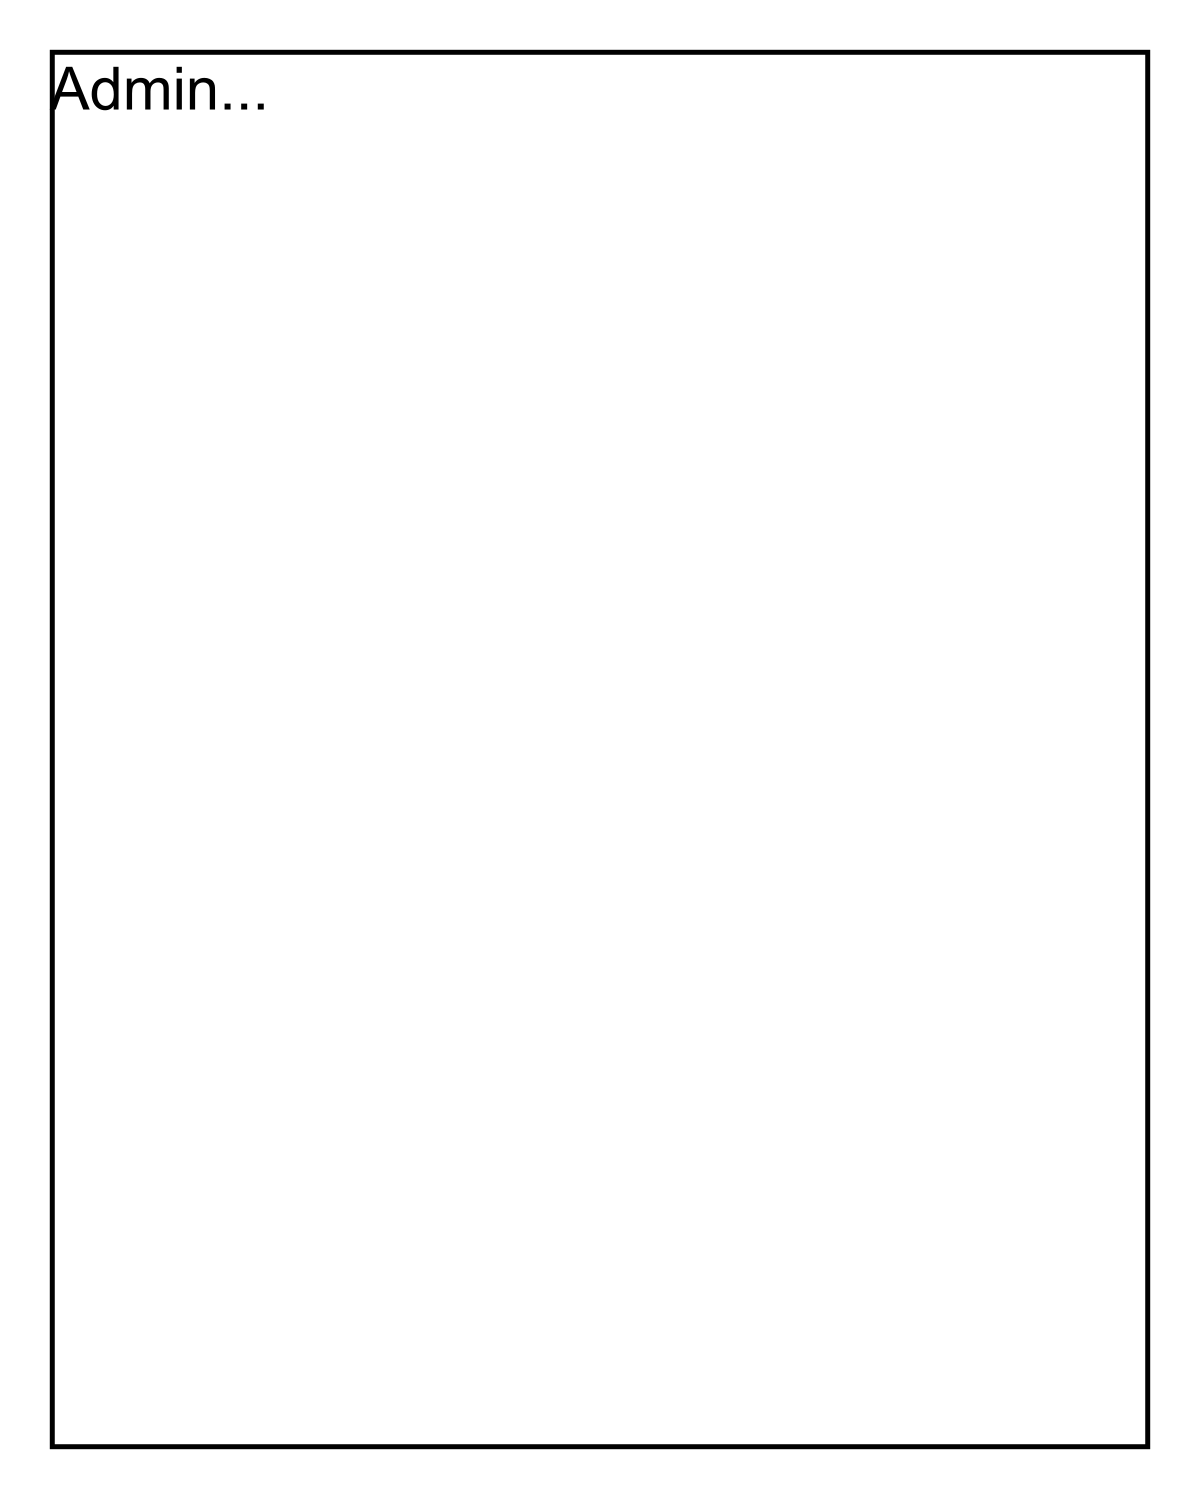
\includegraphics[width=0.5\textwidth]{Images/chapter_26/section_5683148496306176/5905668467720192.png}
 \caption{The Admin class}
\end{figure}

\textbf{R1:} The system shall allow the admin to add or update players, teams, tournaments, and match statistics.

\subsubsection{Run, ball, and wicket}\label{qArAzpazExSpRVBKU0guE}
\\
The \texttt{Run} class records the number and type of runs scored on a ball. The
\texttt{Ball} class records every detail of a ball, such as the number of runs scored and whether it was a wicket-taking ball. The
\texttt{Wicket} class records the details of the wicket, including its type, the bowler, and the batsman who was declared out.
\\
The mentioned classes are shown below:

\begin{figure}[htbp]
 \centering
 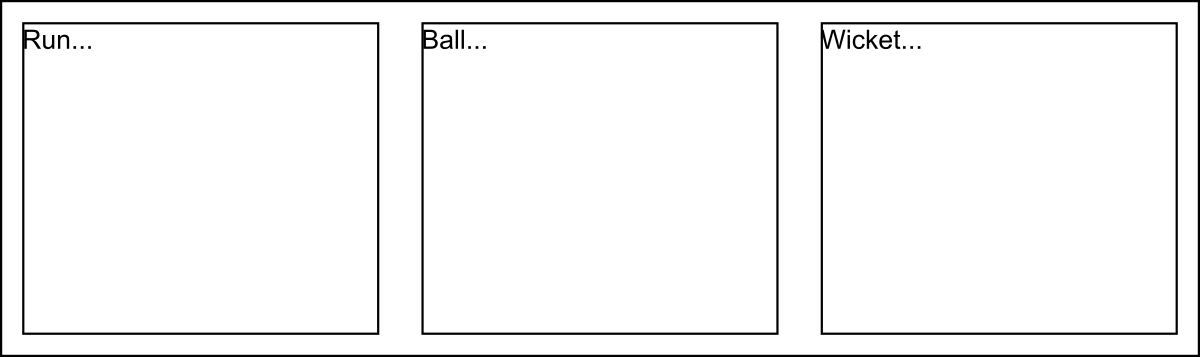
\includegraphics[width=0.5\textwidth]{Images/chapter_26/section_5683148496306176/6533757801857024.png}
 \caption{The Run, Ball, and Wicket classes}
\end{figure}

\textbf{R2:} The system shall enable the commentator to add or modify ball-by-ball commentary, and allow tracking of every score or wicket per ball.

\subsubsection{Over and innings}\label{CKT4bOXGmvktHc5BsQ_rN}
\\
The \texttt{Over} class represents all the details of an over of the innings. The
\texttt{Innings} class represents the details of a match innings. The two classes are shown below:

\begin{figure}[htbp]
 \centering
 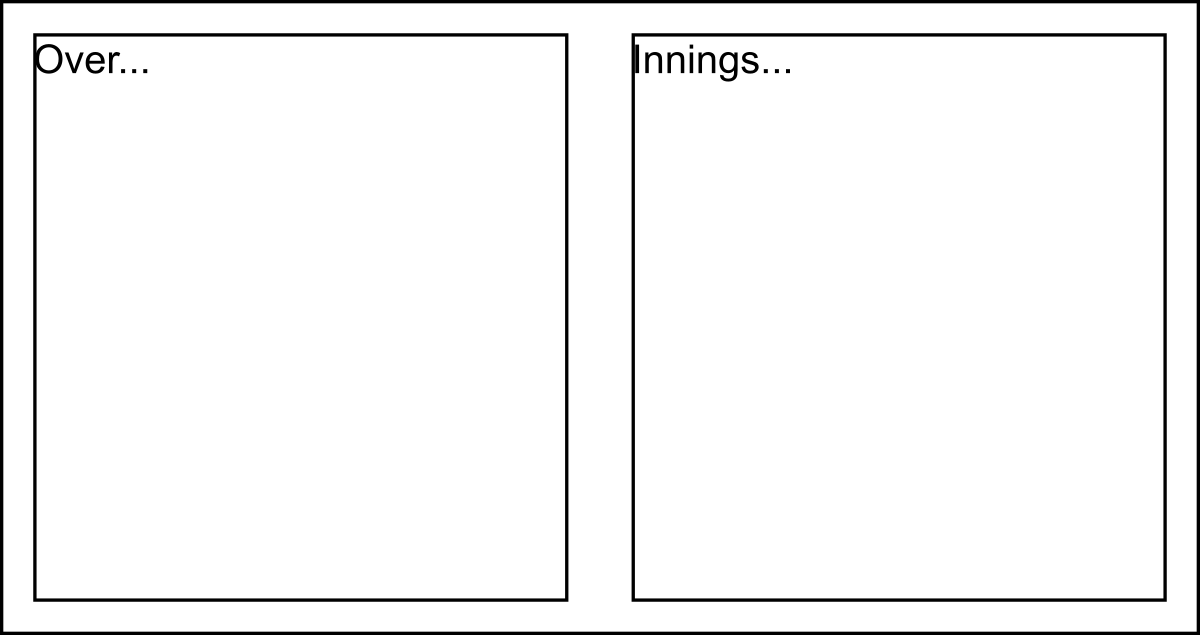
\includegraphics[width=0.5\textwidth]{Images/chapter_26/section_5683148496306176/4811278515437568.png}
 \caption{The Over and Innings classes}
\end{figure}

\subsubsection{Match}\label{3jhOL4s49jmNZB6VJrkuf}
\\
The \texttt{Match} class is an abstract class that has three child classes, representing the types of matches that can occur.

\begin{itemize}
\item
\protect\phantomsection\label{wacaLJjjX6PevJSXbN3BO}
The \texttt{Test} class
\item
\protect\phantomsection\label{X5gzPFRKeRGQrfnGKEt3F}
The \texttt{ODI} class
\item
\protect\phantomsection\label{Jq_Yq5EO2eMtVvjqcTW5B}
The \texttt{T20} class
\end{itemize}
\\
The class diagram is shown below:

\begin{figure}[htbp]
 \centering
 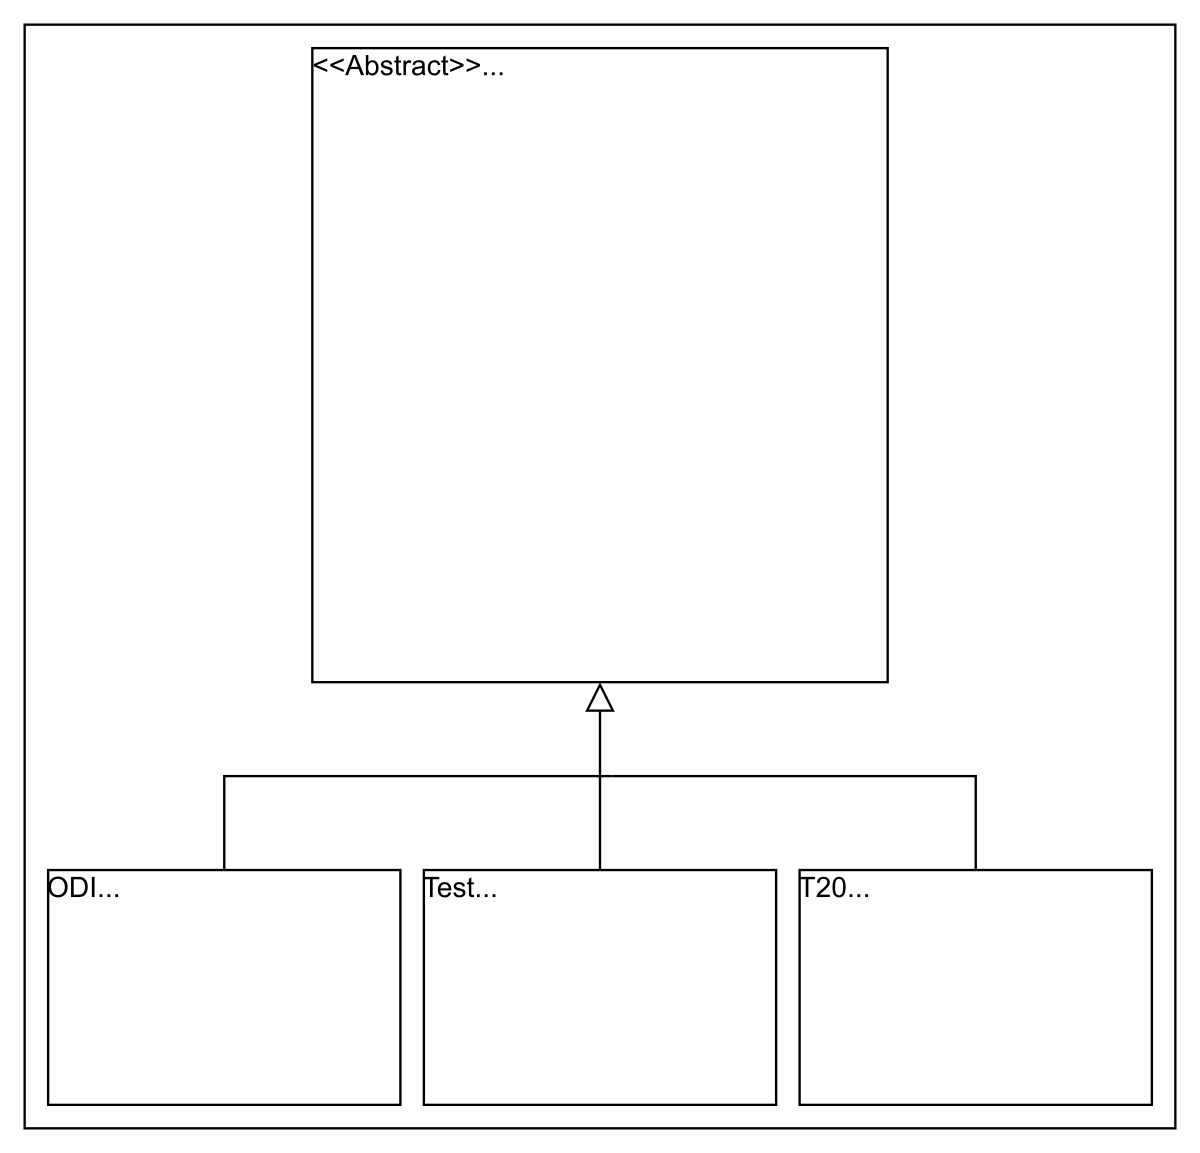
\includegraphics[width=0.5\textwidth]{Images/chapter_26/section_5683148496306176/4871672271077376.png}
 \caption{The Match and its derived classes}
\end{figure}

\textbf{R3:} The system shall support tracking all matches, including Test, ODI, and T20, added or modified by the admin.

\subsubsection{Stadium}\label{prbB31IcYp_mp1fXf84Mi}
\\
The \texttt{Stadium} class represents the information about a stadium, including its name, address, and capacity. The UML representation of this class is given below:

\begin{figure}[htbp]
 \centering
 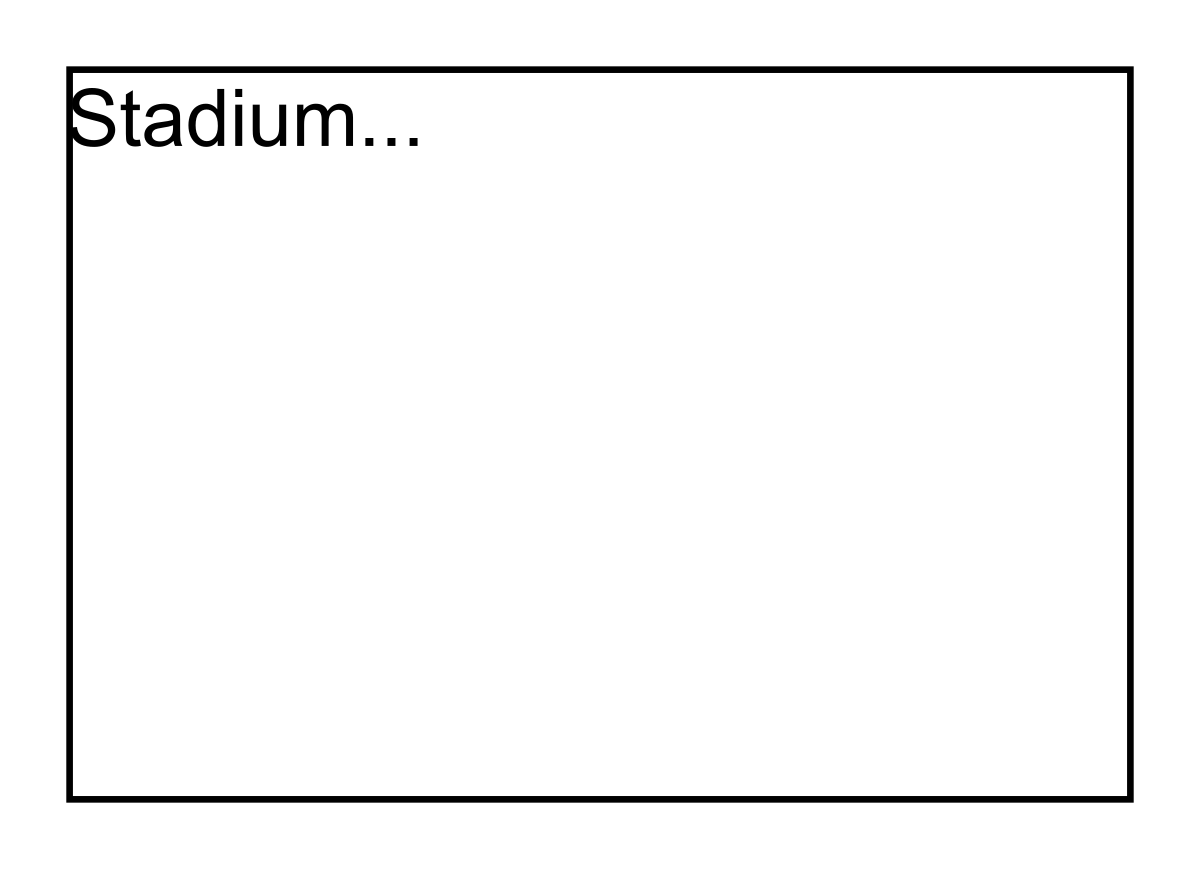
\includegraphics[width=0.5\textwidth]{Images/chapter_26/section_5683148496306176/5211031084072960.png}
 \caption{The Stadium class}
\end{figure}

\subsubsection{Player, coach, and umpire}\label{fBeN52mVi0sYlRWIXd6iq}
\\
The \texttt{Player} class includes the information of a player and their statistics. The
\texttt{Coach} class contains the information of a coach. The
\texttt{Umpire} class contains the information of an umpire. The three classes are shown below:

\begin{figure}[htbp]
 \centering
 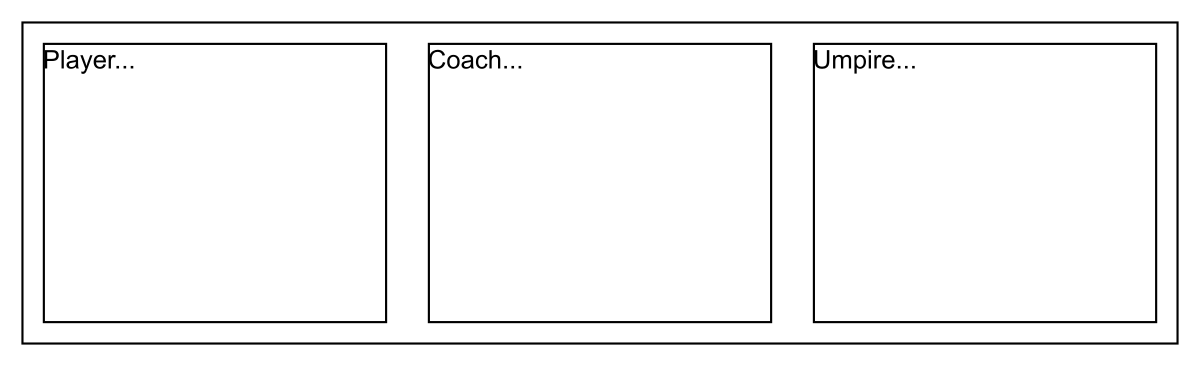
\includegraphics[width=0.5\textwidth]{Images/chapter_26/section_5683148496306176/6090542449295360.png}
 \caption{The Player, Coach, and Umpire classes}
\end{figure}

\textbf{R6:} The system will allow the coach to submit a tournament squad---a group of selected players eligible to participate.
\\
\textbf{R8:} The admin shall be able to manage the entire system by adding or modifying tournaments, matches, teams, players, stadiums, umpires, commentators, and updating stats and news.

\subsubsection{Team, tournament squad, and playing eleven}\label{dNN4pRkxtG9m94dDruSim}
\\
The \texttt{Team} class represents the information about a cricket team, including the list of players, the team coach, and any news related to the team.
\\
The \texttt{TournamentSquad} class represents the team members participating in a tournament. The
\texttt{Playing11} class represents the squad members playing in a match.
\\
The class diagram for these classes is given below:

\begin{figure}[htbp]
 \centering
 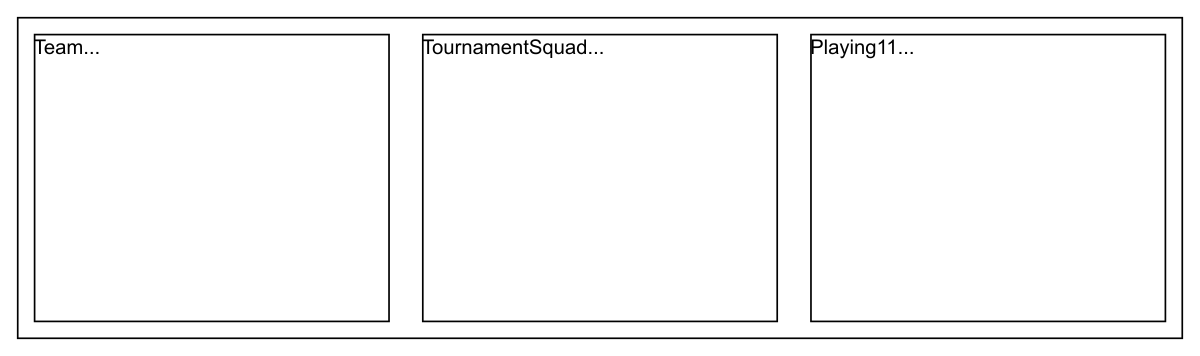
\includegraphics[width=0.5\textwidth]{Images/chapter_26/section_5683148496306176/6593596424585216.png}
 \caption{The Team, TournamentSquad, and Playing11 classes}
\end{figure}

\textbf{R7:} The system shall support playing eleven selections from the tournament squad for each match. Although not directly modeled as a use case, this process is implicit in match setup and should be facilitated by the admin or coach through data entry.

\subsubsection{Tournament and points table}\label{f-nmebJWg_vsqWteRsUy5}
\\
The \texttt{Tournament} class contains information about a cricket tournament. The
\texttt{PointsTable} class displays the accumulated points and match results of the teams participating in the tournament. These classes are shown below:

\begin{figure}[htbp]
 \centering
 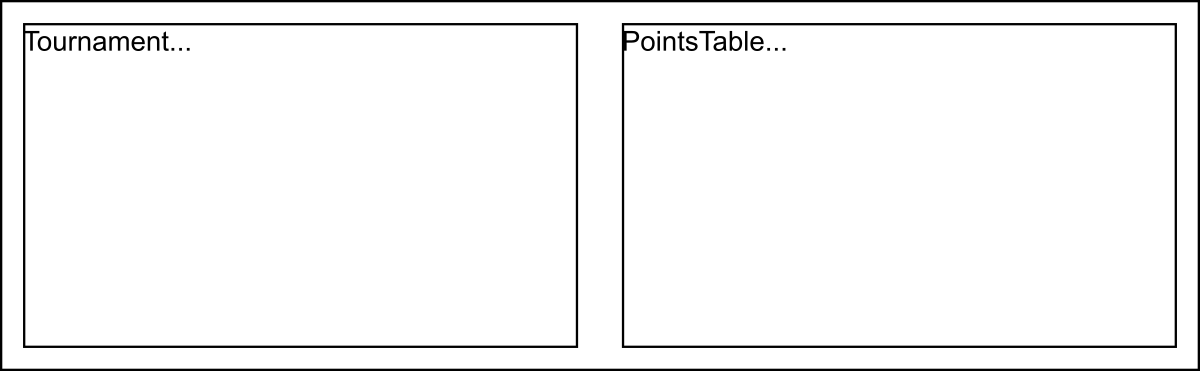
\includegraphics[width=0.5\textwidth]{Images/chapter_26/section_5683148496306176/6584658600132608.png}
 \caption{The Tournament and PointsTable classes}
\end{figure}

\textbf{R4:} The system shall maintain a record of ongoing and historical tournaments and display points tables for all participating teams. The admin is responsible for adding or updating tournaments.

\subsubsection{Stats}\label{KdqcCcB6eP_AQF4yhNlUz}
\\
The \texttt{Stat} class is an abstract class that extends to \texttt{PlayerStat}, \texttt{TeamStat}, and \texttt{MatchStat} classes. These classes contain important statistics. The UML representation is shown below:

\begin{figure}[htbp]
 \centering
 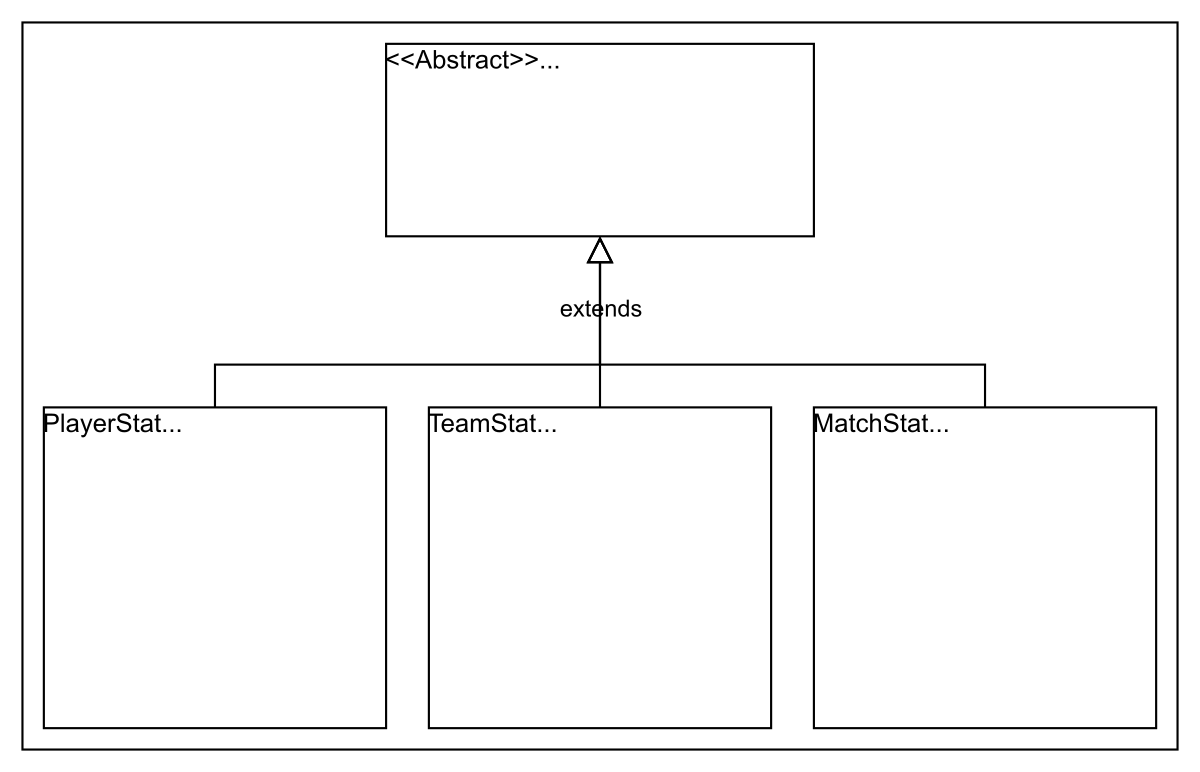
\includegraphics[width=0.5\textwidth]{Images/chapter_26/section_5683148496306176/5421089990508544.png}
 \caption{Stat and its derived classes}
\end{figure}

\textbf{R8:} The admin shall be able to manage the entire system by adding or modifying tournaments, matches, teams, players, stadiums, umpires, commentators, and updating stats and news.

\subsubsection{Commentator and commentary}\label{IIJp11b_U5FfrWdW7QExl}
\\
The \texttt{Commentator} class records the information about the commentator. The
\texttt{Commentary} class contains information about the commentary for every ball of an over. The two classes are shown below:

\begin{figure}[htbp]
 \centering
 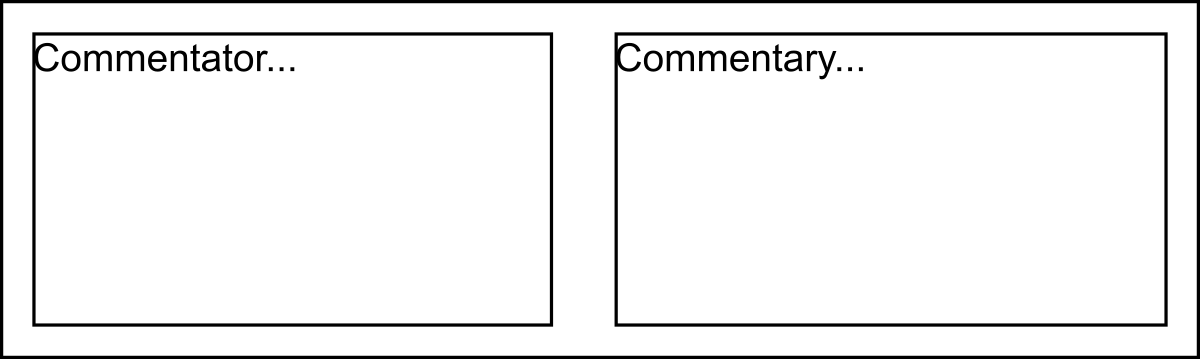
\includegraphics[width=0.5\textwidth]{Images/chapter_26/section_5683148496306176/5018460322267136.png}
 \caption{The Commentator and Commentary classes}
\end{figure}

\textbf{R2:} The system shall enable the commentator to add or modify ball-by-ball commentary, and allow tracking of every score or wicket per ball.

\subsubsection{News}\label{r-nmVnouXH6tT_HnUIA5m}
\\
The \texttt{News} class holds the news updates of a team. The definition of this class is given below:

\begin{figure}[htbp]
 \centering
 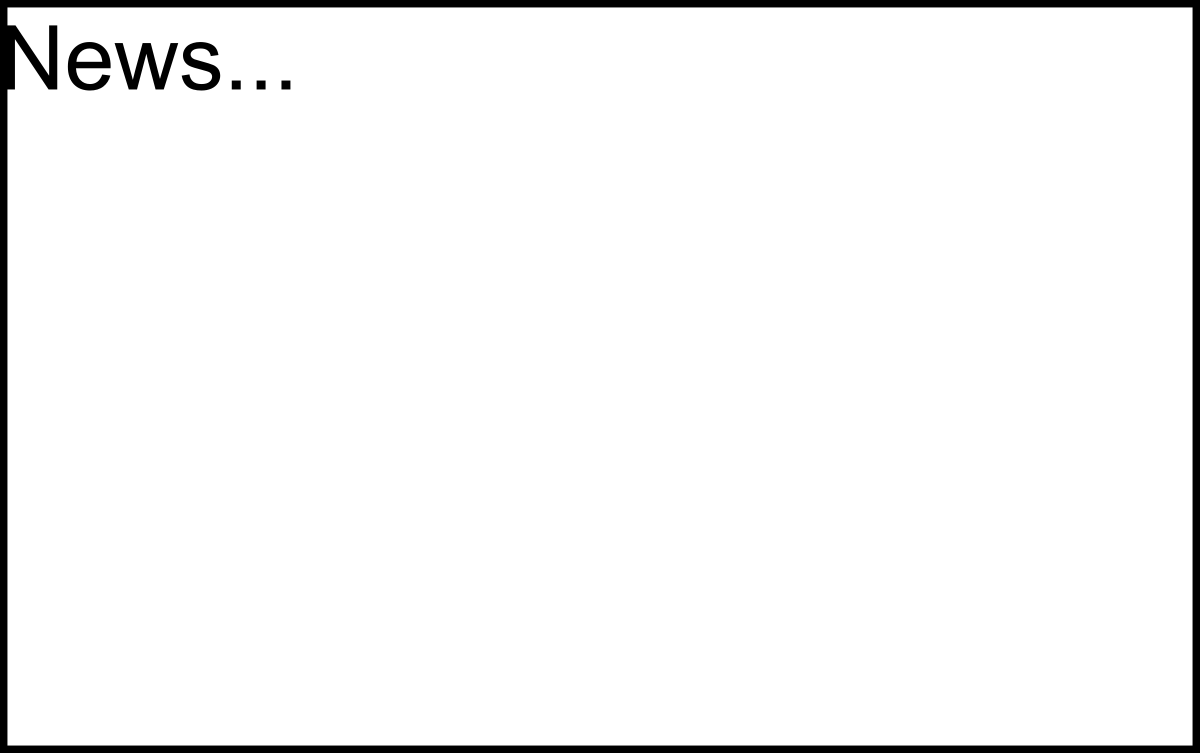
\includegraphics[width=0.5\textwidth]{Images/chapter_26/section_5683148496306176/5174113829388288.png}
 \caption{The News class}
\end{figure}

\subsubsection{Enumerations}\label{PDS8aQ81vAReYwxGo6J8q}
\\
The enumerations required in the ESPNcricinfo system are listed below:

\begin{itemize}
\item
\protect\phantomsection\label{2hAlzl4hYF_zQuqNrafEg}
\texttt{MatchResult}\textbf{:} This records the result of a match---a win, loss, canceled, or draw.
\item
\protect\phantomsection\label{dYsIhqOptZnkQBFgfSGpK}
\texttt{UmpireType}\textbf{:} This records the type of umpire---field umpire, third umpire, or reserved.
\item
\protect\phantomsection\label{uufu_oV_hg_5DvlLOCYEu}
\texttt{WicketType}\textbf{:} This records the type of the wicket---stumped, bowled, caught, etc.
\item
\protect\phantomsection\label{f0zqy6qxyXp-_0Lv1gzR8}
\texttt{BallType}\textbf{:} This records the type of ball played---a regular delivery, wide, no ball, or wicket.
\item
\protect\phantomsection\label{S65pDeZjAhX7SFk80wfwZ}
\texttt{RunType}\textbf{:} This records the type of run scored---a regular run, four, six, wide, etc.
\item
\protect\phantomsection\label{1OI2qvbkye1FOOoDuePsW}
\texttt{PlayingPosition}\textbf{:} This records the playing position of a player---batsman, bowler, or all-rounder.
\end{itemize}

\begin{figure}[htbp]
 \centering
 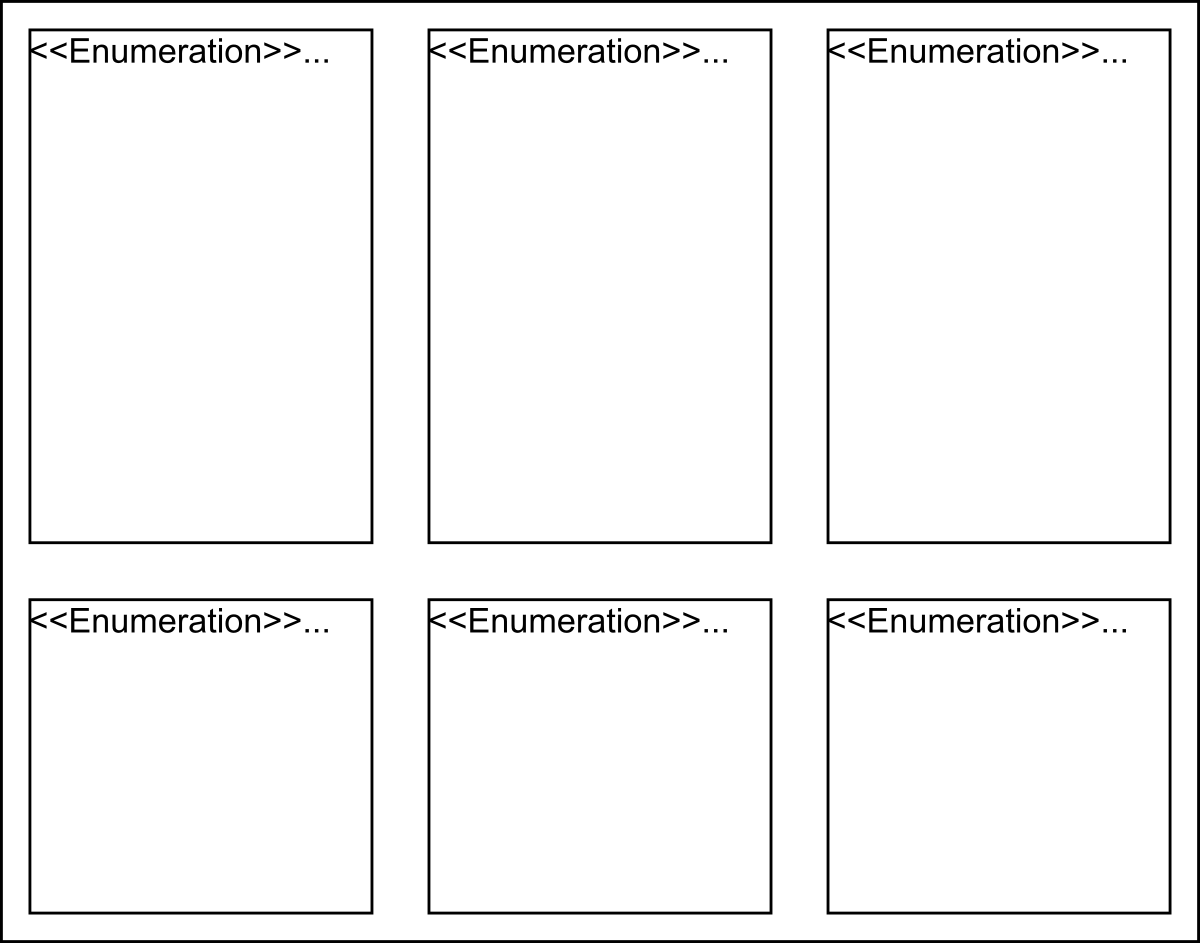
\includegraphics[width=0.5\textwidth]{Images/chapter_26/section_5683148496306176/6123272141012992.png}
 \caption{Enums in ESPNcricinfo}
\end{figure}

\subsubsection{Custom data type}\label{lTyS10KH9L-rbByY7D4cl}
\\
We need to create a custom data type,~\texttt{Address}, that will store the physical location of any place.

\begin{figure}[htbp]
 \centering
 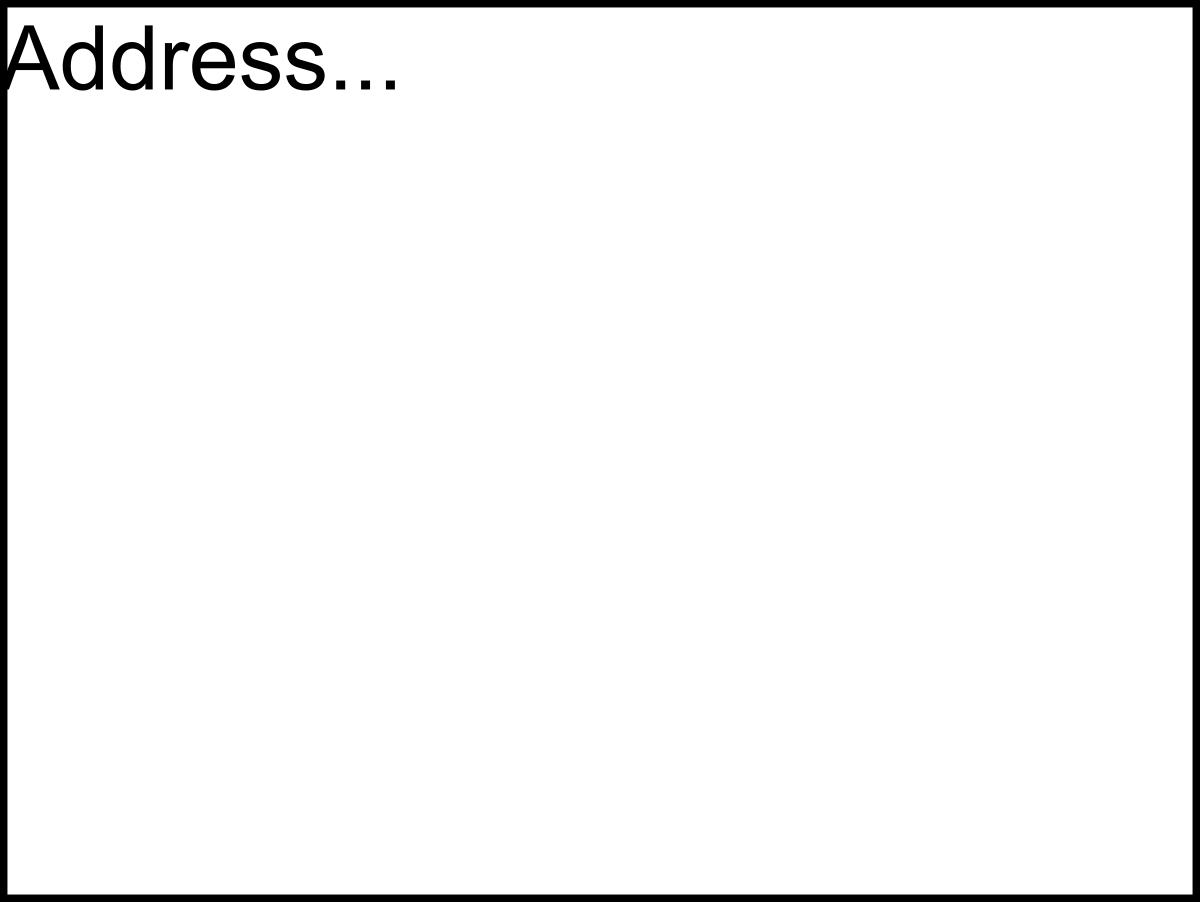
\includegraphics[width=0.5\textwidth]{Images/chapter_26/section_5683148496306176/6399722842357760.png}
 \caption{The Address custom data type}
\end{figure}

\subsection{Relationship between classes}\label{CsdqZ2X_kNb6SUOMEaQcU}
\\
Now, we will discuss the relationships between the classes we have defined above in our ESPNcricinfo system.

\subsubsection{Association}\label{LZd7fmUfc9JcRnHlG4hg0}
\\
The class diagram has the following association relationships:
\\
\paragraph{One-way association}\label{HtaSB-7SLOrz6NIXCWAop}

\begin{itemize}
\item
\protect\phantomsection\label{hTpEg7o6T3qKkk_BQouaw}
The \texttt{Admin} class has a one-way association with the \texttt{Player}, \texttt{Team}, \texttt{Match}, and \texttt{Tournament} classes.
\item
\protect\phantomsection\label{DYzF7u0zp2UH-1yzcRzvs}
The \texttt{Player} class has a one-way association with the \texttt{Run}, \texttt{Ball}, \texttt{Wicket}, and \texttt{Over} classes.
\item
\protect\phantomsection\label{atvPAal5_a88_tFrGyX2_}
The \texttt{Team} class has a one-way association with the \texttt{TournamentSquad} and \texttt{Tournament} classes.
\item
\protect\phantomsection\label{9OPJPQUtZrJh6vmSrd5K_}
The \texttt{TournamentSquad} class has a one-way association with the \texttt{Playing11} class.
\end{itemize}
\\
\paragraph{Two-way association}\label{GUVn9O93ioQZ7owKg6pBJ}

\begin{itemize}
\item
\protect\phantomsection\label{GOIVLgtpjvoM5MCRzrtV3}
The \texttt{Ball} class is associated with the \texttt{Run}, \texttt{Wicket}, and \texttt{Commentary} classes.
\item
\protect\phantomsection\label{seEOPXyZjT_61pSC-a5VW}
The \texttt{Team} class is associated with the \texttt{Coach} and \texttt{News} classes.
\item
\protect\phantomsection\label{Bk0Ucxhl6w9-GtEcX_DPS}
The \texttt{Commentary} class is associated with the \texttt{Commentator} class.
\item
\protect\phantomsection\label{2BUcqY_Y1viPg8aHYB4t5}
The \texttt{Match} class is associated with the \texttt{Umpire}, \texttt{Commentator}, \texttt{News}, and \texttt{Stadium} classes.
\item
\protect\phantomsection\label{seEOPXyZjT_61pSC-a5VW}
The \texttt{Player} class is associated with the \texttt{News} classes.
\end{itemize}

\begin{figure}[htbp]
 \centering
 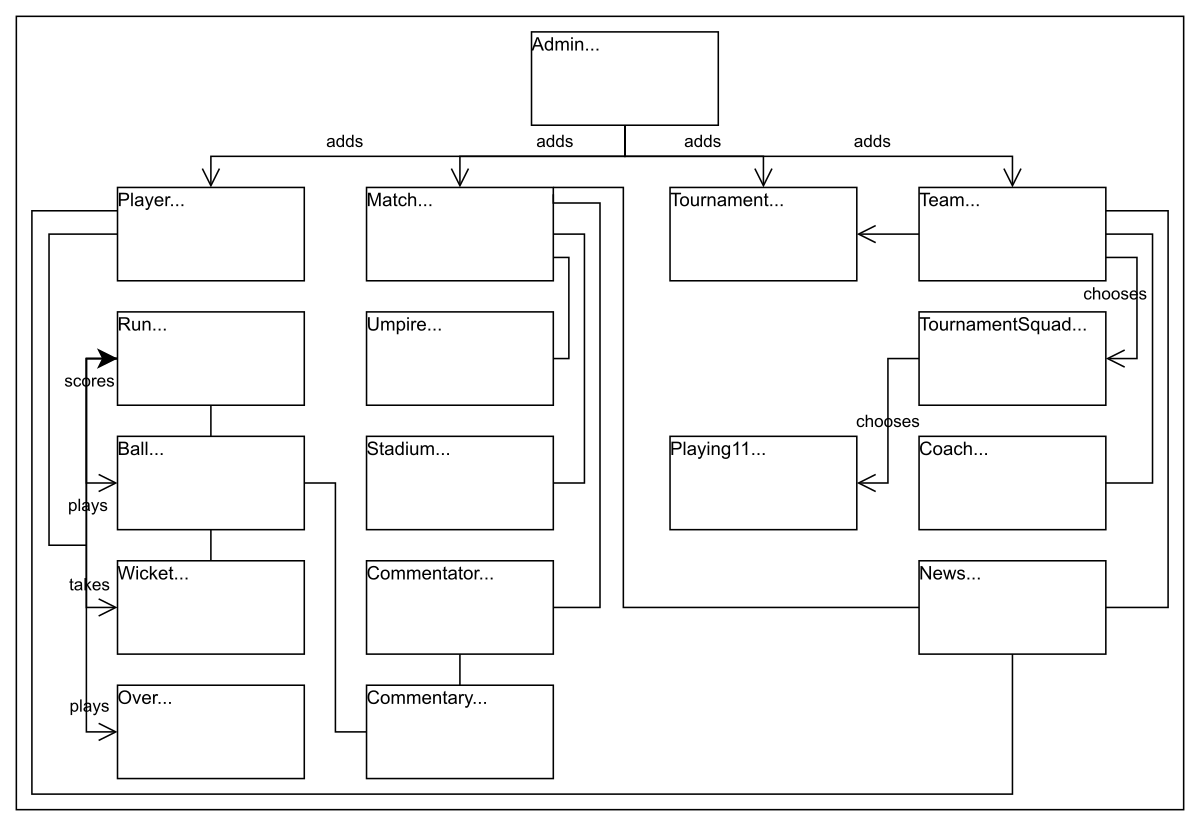
\includegraphics[width=0.5\textwidth]{Images/chapter_26/section_5683148496306176/4615569746558976.png}
 \caption{The association relationships between classes}
\end{figure}

\subsubsection{Aggregation}\label{45LcDLiSznd6EK4EGEcIu}
\\
The class diagram has the following aggregation relationships:

\begin{itemize}
\item
\protect\phantomsection\label{pAgjWurG4Dq6ppkdaUuNA}
The \texttt{Tournament} class contains the \texttt{TournamentSquad} class.
\end{itemize}

\begin{figure}[htbp]
 \centering
 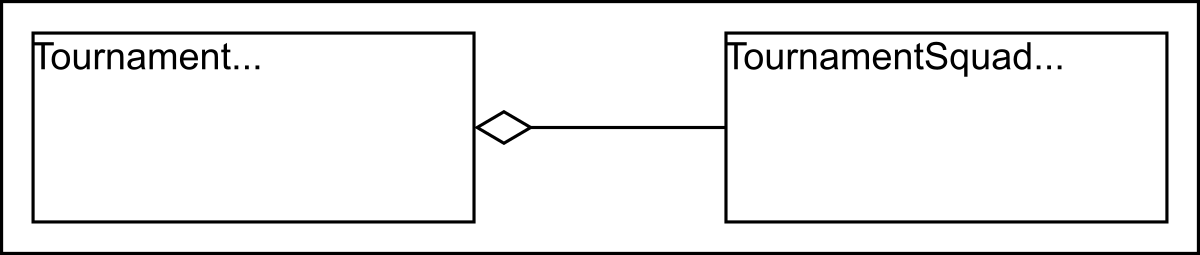
\includegraphics[width=0.5\textwidth]{Images/chapter_26/section_5683148496306176/5542068190707712.png}
 \caption{The aggregation relationship between classes}
\end{figure}

\subsubsection{Composition}\label{oAyS25a2hiUul4YPEvg3I}
\\
The class diagram has the following composition relationships:

\begin{itemize}
\item
\protect\phantomsection\label{EqNzqkqJjwUfLiPIpNb61}
The \texttt{Player} class is composed of the \texttt{PlayerStat} class.
\item
\protect\phantomsection\label{4suKJNxls4qlJbOLKPhqj}
The \texttt{Team} class is composed of the \texttt{Player} and \texttt{TeamStat} classes.
\item
\protect\phantomsection\label{wXTWtF8XnYEy4X6ybxhmR}
The \texttt{Tournament} class is composed of the \texttt{Match} and \texttt{PointsTable} classes.
\item
\protect\phantomsection\label{cOB-PlYcWeRGIrXV8a47X}
The \texttt{Match} class is composed of the \texttt{Playing11}, \texttt{Innings}, and \texttt{MatchStat} classes.
\item
\protect\phantomsection\label{_fOj48tKLgamP0wN1I8DO}
The \texttt{Innings} class is composed of the \texttt{Over} class.
\item
\protect\phantomsection\label{0DOIOlK4XPlafrgVqfdHp}
The \texttt{Over} class is composed of the \texttt{Ball} class.
\end{itemize}

\begin{figure}[htbp]
 \centering
 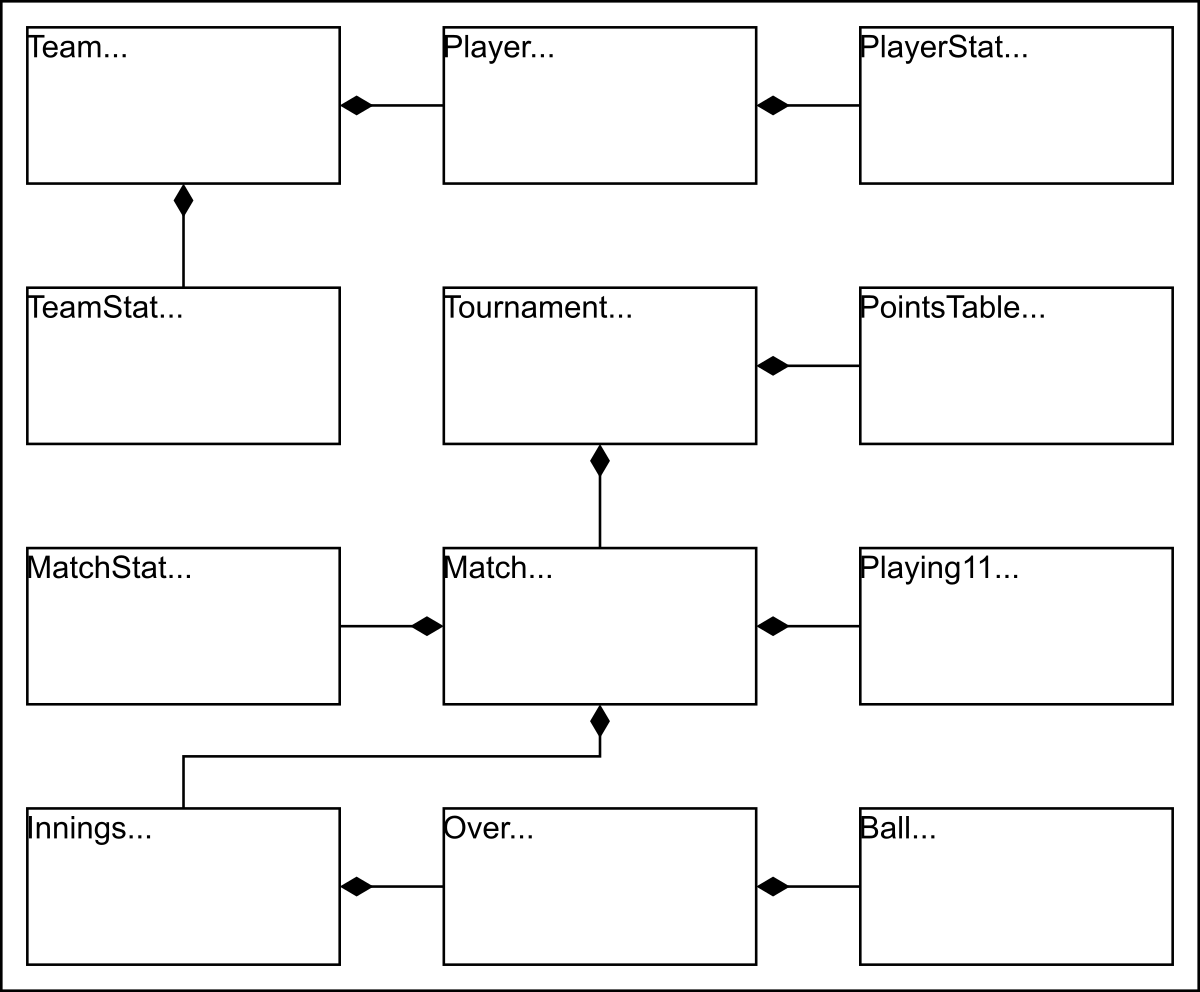
\includegraphics[width=0.5\textwidth]{Images/chapter_26/section_5683148496306176/6274289700700160.png}
 \caption{The composition relationships between classes}
\end{figure}

\subsubsection{Inheritance}\label{3DIxUvsdYCX5fRXWrL0I7}
\\
The class diagram has the following inheritance relationships:

\begin{itemize}
\item
\protect\phantomsection\label{yEK3EQ5YW4CX_qQpc8hJv}
The \texttt{ODI}, \texttt{Test}, and \texttt{T20} classes are derived from the \texttt{Match} class.
\item
\protect\phantomsection\label{k1YV635vwwZXy5flLWuid}
The \texttt{TeamStat}, \texttt{MatchStat}, and \texttt{PlayerStat} classes are derived from the \texttt{Stat} class.
\end{itemize}
\begin{quote}
\textbf{Note:} We have already discussed the inheritance relationship between classes in the component section above one by one.
\end{quote}
\subsection{Class diagram of ESPNcricinfo}\label{NoJQhNYaUQtOBPi_fkMyV}
\\
In this section, we outline the multiplicity (cardinality) relationships between the main classes in our~ESPNcricinfo system. For each relationship, we explain the allowed number of instances on each side and the real-world or design rationale behind the connection. Understanding these relationships is key to modeling how different entities interact and collaborate to support key workflows in the system.

\begin{center}
{\def\LTcaptype{none} % do not increment counter
\begin{longtable}[]{@{}
>{\raggedright\arraybackslash} p{(\linewidth - 6\tabcolsep) * \real{0.2500}}
>{\raggedright\arraybackslash} p{(\linewidth - 6\tabcolsep) * \real{0.2500}}
>{\raggedright\arraybackslash} p{(\linewidth - 6\tabcolsep) * \real{0.2500}}
>{\raggedright\arraybackslash} p{(\linewidth - 6\tabcolsep) * \real{0.2500}}@{}}
\toprule\noalign{}
\endhead
\bottomrule\noalign{}
\endlastfoot
\begin{minipage}[t]{\linewidth}\raggedright
\textbf{Source}
\end{minipage} & \begin{minipage}[t]{\linewidth}\raggedright
\textbf{Target}
\end{minipage} & \begin{minipage}[t]{\linewidth}\raggedright
\textbf{Multiplicity}
\end{minipage} & \begin{minipage}[t]{\linewidth}\raggedright
\textbf{Description}
\end{minipage} \\
\begin{minipage}[t]{\linewidth}\raggedright
Player
\end{minipage} & \begin{minipage}[t]{\linewidth}\raggedright
Run
\end{minipage} & \begin{minipage}[t]{\linewidth}\raggedright
1 -- 0..*
\end{minipage} & \begin{minipage}[t]{\linewidth}\raggedright
A player can score multiple runs
\end{minipage} \\
\begin{minipage}[t]{\linewidth}\raggedright
Player
\end{minipage} & \begin{minipage}[t]{\linewidth}\raggedright
Wicket
\end{minipage} & \begin{minipage}[t]{\linewidth}\raggedright
1 -- 0..*
\end{minipage} & \begin{minipage}[t]{\linewidth}\raggedright
A player can be involved in multiple wickets
\end{minipage} \\
\begin{minipage}[t]{\linewidth}\raggedright
Ball
\end{minipage} & \begin{minipage}[t]{\linewidth}\raggedright
Run
\end{minipage} & \begin{minipage}[t]{\linewidth}\raggedright
1 -- 0..*
\end{minipage} & \begin{minipage}[t]{\linewidth}\raggedright
A ball can result in multiple runs
\end{minipage} \\
\begin{minipage}[t]{\linewidth}\raggedright
Ball
\end{minipage} & \begin{minipage}[t]{\linewidth}\raggedright
Wicket
\end{minipage} & \begin{minipage}[t]{\linewidth}\raggedright
1 -- 0..1
\end{minipage} & \begin{minipage}[t]{\linewidth}\raggedright
A ball can result in zero or one wicket
\end{minipage} \\
\begin{minipage}[t]{\linewidth}\raggedright
Ball
\end{minipage} & \begin{minipage}[t]{\linewidth}\raggedright
Player
\end{minipage} & \begin{minipage}[t]{\linewidth}\raggedright
1 -- 2
\end{minipage} & \begin{minipage}[t]{\linewidth}\raggedright
Each ball has a bowler and a batsman
\end{minipage} \\
\begin{minipage}[t]{\linewidth}\raggedright
Over
\end{minipage} & \begin{minipage}[t]{\linewidth}\raggedright
Ball
\end{minipage} & \begin{minipage}[t]{\linewidth}\raggedright
1 -- 0..*
\end{minipage} & \begin{minipage}[t]{\linewidth}\raggedright
An over can have multiple balls
\end{minipage} \\
\begin{minipage}[t]{\linewidth}\raggedright
Over
\end{minipage} & \begin{minipage}[t]{\linewidth}\raggedright
Player
\end{minipage} & \begin{minipage}[t]{\linewidth}\raggedright
1 -- 1
\end{minipage} & \begin{minipage}[t]{\linewidth}\raggedright
One player bowls each over
\end{minipage} \\
\begin{minipage}[t]{\linewidth}\raggedright
Innings
\end{minipage} & \begin{minipage}[t]{\linewidth}\raggedright
Over
\end{minipage} & \begin{minipage}[t]{\linewidth}\raggedright
1 -- 0..*
\end{minipage} & \begin{minipage}[t]{\linewidth}\raggedright
Each innings can have multiple overs
\end{minipage} \\
\begin{minipage}[t]{\linewidth}\raggedright
Innings
\end{minipage} & \begin{minipage}[t]{\linewidth}\raggedright
Playing11
\end{minipage} & \begin{minipage}[t]{\linewidth}\raggedright
1 -- 2
\end{minipage} & \begin{minipage}[t]{\linewidth}\raggedright
Each innings has one batting and one bowling team
\end{minipage} \\
\begin{minipage}[t]{\linewidth}\raggedright
Match
\end{minipage} & \begin{minipage}[t]{\linewidth}\raggedright
Innings
\end{minipage} & \begin{minipage}[t]{\linewidth}\raggedright
1 -- 0..*
\end{minipage} & \begin{minipage}[t]{\linewidth}\raggedright
Each match can have multiple innings
\end{minipage} \\
\begin{minipage}[t]{\linewidth}\raggedright
Match
\end{minipage} & \begin{minipage}[t]{\linewidth}\raggedright
Team
\end{minipage} & \begin{minipage}[t]{\linewidth}\raggedright
1 -- 2
\end{minipage} & \begin{minipage}[t]{\linewidth}\raggedright
Each match involves two teams
\end{minipage} \\
\begin{minipage}[t]{\linewidth}\raggedright
Match
\end{minipage} & \begin{minipage}[t]{\linewidth}\raggedright
Stadium
\end{minipage} & \begin{minipage}[t]{\linewidth}\raggedright
1 -- 1
\end{minipage} & \begin{minipage}[t]{\linewidth}\raggedright
Each match is played in one stadium
\end{minipage} \\
\begin{minipage}[t]{\linewidth}\raggedright
Match
\end{minipage} & \begin{minipage}[t]{\linewidth}\raggedright
Umpire
\end{minipage} & \begin{minipage}[t]{\linewidth}\raggedright
1 -- 2..4
\end{minipage} & \begin{minipage}[t]{\linewidth}\raggedright
Each match can have 2 to 4 umpires
\end{minipage} \\
\begin{minipage}[t]{\linewidth}\raggedright
Match
\end{minipage} & \begin{minipage}[t]{\linewidth}\raggedright
Commentator
\end{minipage} & \begin{minipage}[t]{\linewidth}\raggedright
1 -- 0..*
\end{minipage} & \begin{minipage}[t]{\linewidth}\raggedright
Each match can have multiple commentators
\end{minipage} \\
\begin{minipage}[t]{\linewidth}\raggedright
Match
\end{minipage} & \begin{minipage}[t]{\linewidth}\raggedright
MatchStat
\end{minipage} & \begin{minipage}[t]{\linewidth}\raggedright
1 -- 1
\end{minipage} & \begin{minipage}[t]{\linewidth}\raggedright
Each match has one match statistics record
\end{minipage} \\
\begin{minipage}[t]{\linewidth}\raggedright
Team
\end{minipage} & \begin{minipage}[t]{\linewidth}\raggedright
Player
\end{minipage} & \begin{minipage}[t]{\linewidth}\raggedright
1 -- 0..*
\end{minipage} & \begin{minipage}[t]{\linewidth}\raggedright
A team can have multiple players
\end{minipage} \\
\begin{minipage}[t]{\linewidth}\raggedright
Team
\end{minipage} & \begin{minipage}[t]{\linewidth}\raggedright
Coach
\end{minipage} & \begin{minipage}[t]{\linewidth}\raggedright
1 -- 1
\end{minipage} & \begin{minipage}[t]{\linewidth}\raggedright
Each team has one coach
\end{minipage} \\
\begin{minipage}[t]{\linewidth}\raggedright
Team
\end{minipage} & \begin{minipage}[t]{\linewidth}\raggedright
News
\end{minipage} & \begin{minipage}[t]{\linewidth}\raggedright
1 -- 0..*
\end{minipage} & \begin{minipage}[t]{\linewidth}\raggedright
A team can have multiple news entries
\end{minipage} \\
\begin{minipage}[t]{\linewidth}\raggedright
Team
\end{minipage} & \begin{minipage}[t]{\linewidth}\raggedright
TeamStat
\end{minipage} & \begin{minipage}[t]{\linewidth}\raggedright
1 -- 1
\end{minipage} & \begin{minipage}[t]{\linewidth}\raggedright
Each team has one statistics record
\end{minipage} \\
\begin{minipage}[t]{\linewidth}\raggedright
Tournament
\end{minipage} & \begin{minipage}[t]{\linewidth}\raggedright
Match
\end{minipage} & \begin{minipage}[t]{\linewidth}\raggedright
1 -- 0..*
\end{minipage} & \begin{minipage}[t]{\linewidth}\raggedright
A tournament includes multiple matches
\end{minipage} \\
\begin{minipage}[t]{\linewidth}\raggedright
Tournament
\end{minipage} & \begin{minipage}[t]{\linewidth}\raggedright
TournamentSquad
\end{minipage} & \begin{minipage}[t]{\linewidth}\raggedright
1 -- 0..*
\end{minipage} & \begin{minipage}[t]{\linewidth}\raggedright
A tournament has multiple squads
\end{minipage} \\
\begin{minipage}[t]{\linewidth}\raggedright
TournamentSquad
\end{minipage} & \begin{minipage}[t]{\linewidth}\raggedright
Player
\end{minipage} & \begin{minipage}[t]{\linewidth}\raggedright
1 -- 0..*
\end{minipage} & \begin{minipage}[t]{\linewidth}\raggedright
Each tournament squad has multiple players
\end{minipage} \\
\begin{minipage}[t]{\linewidth}\raggedright
TournamentSquad
\end{minipage} & \begin{minipage}[t]{\linewidth}\raggedright
Tournament
\end{minipage} & \begin{minipage}[t]{\linewidth}\raggedright
0..* -- 1
\end{minipage} & \begin{minipage}[t]{\linewidth}\raggedright
Each tournament squad belongs to one tournament
\end{minipage} \\
\begin{minipage}[t]{\linewidth}\raggedright
Playing11
\end{minipage} & \begin{minipage}[t]{\linewidth}\raggedright
Player
\end{minipage} & \begin{minipage}[t]{\linewidth}\raggedright
1 -- 0..*
\end{minipage} & \begin{minipage}[t]{\linewidth}\raggedright
A playing eleven contains multiple players
\end{minipage} \\
\begin{minipage}[t]{\linewidth}\raggedright
Commentary
\end{minipage} & \begin{minipage}[t]{\linewidth}\raggedright
Commentator
\end{minipage} & \begin{minipage}[t]{\linewidth}\raggedright
1 -- 1
\end{minipage} & \begin{minipage}[t]{\linewidth}\raggedright
One commentator gives each commentary
\end{minipage} \\
\begin{minipage}[t]{\linewidth}\raggedright
News
\end{minipage} & \begin{minipage}[t]{\linewidth}\raggedright
Team
\end{minipage} & \begin{minipage}[t]{\linewidth}\raggedright
1 -- 1
\end{minipage} & \begin{minipage}[t]{\linewidth}\raggedright
Each news item is linked to one team
\end{minipage} \\
\begin{minipage}[t]{\linewidth}\raggedright
Admin
\end{minipage} & \begin{minipage}[t]{\linewidth}\raggedright
Player
\end{minipage} & \begin{minipage}[t]{\linewidth}\raggedright
1 -- 0..*
\end{minipage} & \begin{minipage}[t]{\linewidth}\raggedright
Admin manages multiple players
\end{minipage} \\
\begin{minipage}[t]{\linewidth}\raggedright
Admin
\end{minipage} & \begin{minipage}[t]{\linewidth}\raggedright
Team
\end{minipage} & \begin{minipage}[t]{\linewidth}\raggedright
1 -- 0..*
\end{minipage} & \begin{minipage}[t]{\linewidth}\raggedright
Admin manages multiple teams
\end{minipage} \\
\begin{minipage}[t]{\linewidth}\raggedright
Admin
\end{minipage} & \begin{minipage}[t]{\linewidth}\raggedright
Coach
\end{minipage} & \begin{minipage}[t]{\linewidth}\raggedright
1 -- 0..*
\end{minipage} & \begin{minipage}[t]{\linewidth}\raggedright
Admin manages multiple coaches
\end{minipage} \\
\begin{minipage}[t]{\linewidth}\raggedright
Admin
\end{minipage} & \begin{minipage}[t]{\linewidth}\raggedright
News
\end{minipage} & \begin{minipage}[t]{\linewidth}\raggedright
1 -- 0..*
\end{minipage} & \begin{minipage}[t]{\linewidth}\raggedright
Admin manages multiple news entries
\end{minipage} \\
\begin{minipage}[t]{\linewidth}\raggedright
Admin
\end{minipage} & \begin{minipage}[t]{\linewidth}\raggedright
Tournament
\end{minipage} & \begin{minipage}[t]{\linewidth}\raggedright
1 -- 0..*
\end{minipage} & \begin{minipage}[t]{\linewidth}\raggedright
Admin manages multiple tournaments
\end{minipage} \\
\begin{minipage}[t]{\linewidth}\raggedright
Admin
\end{minipage} & \begin{minipage}[t]{\linewidth}\raggedright
Match
\end{minipage} & \begin{minipage}[t]{\linewidth}\raggedright
1 -- 0..*
\end{minipage} & \begin{minipage}[t]{\linewidth}\raggedright
Admin manages multiple matches
\end{minipage} \\
\begin{minipage}[t]{\linewidth}\raggedright
Admin
\end{minipage} & \begin{minipage}[t]{\linewidth}\raggedright
Stadium
\end{minipage} & \begin{minipage}[t]{\linewidth}\raggedright
1 -- 0..*
\end{minipage} & \begin{minipage}[t]{\linewidth}\raggedright
Admin manages multiple stadiums
\end{minipage} \\
\begin{minipage}[t]{\linewidth}\raggedright
Admin
\end{minipage} & \begin{minipage}[t]{\linewidth}\raggedright
Umpire
\end{minipage} & \begin{minipage}[t]{\linewidth}\raggedright
1 -- 0..*
\end{minipage} & \begin{minipage}[t]{\linewidth}\raggedright
Admin manages multiple umpires
\end{minipage} \\
\begin{minipage}[t]{\linewidth}\raggedright
Admin
\end{minipage} & \begin{minipage}[t]{\linewidth}\raggedright
Commentator
\end{minipage} & \begin{minipage}[t]{\linewidth}\raggedright
1 -- 0..*
\end{minipage} & \begin{minipage}[t]{\linewidth}\raggedright
Admin manages multiple commentators
\end{minipage} \\
\end{longtable}
}
\end{center}

Here's the complete class diagram for ESPNcricinfo:

\begin{figure}[htbp]
 \centering
 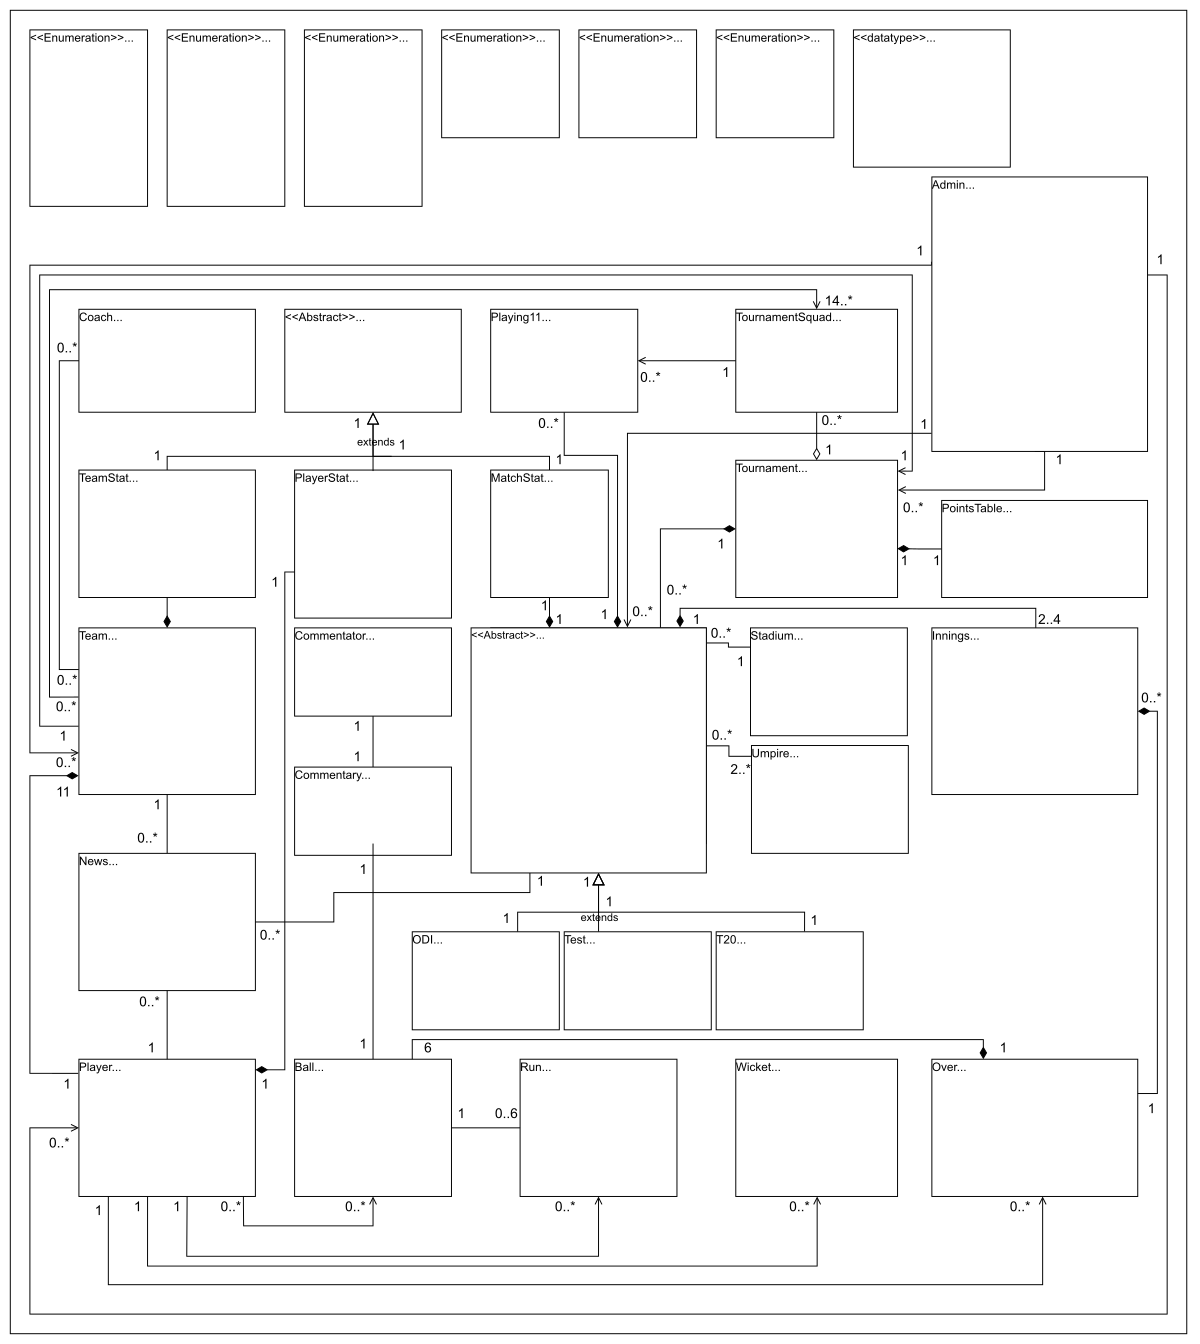
\includegraphics[width=0.5\textwidth]{Images/chapter_26/section_5683148496306176/4802932363886592.png}
 \caption{The class diagram of ESPNcricinfo}
\end{figure}

\subsection{Design pattern}\label{bb0AhxTpVPo6LDk9b1bZd}
\\
To implement ESPNcricinfo's core features in a flexible and scalable way, we apply the object-oriented design patterns based on system behavior.

\begin{itemize}
\item
We know that updates, such as match scores, wickets, or player milestones, can trigger real-time commentary or notifications. To model this behavior, we can use the Observer design pattern.
\item
We recognize that players have different roles, such as batter, bowler, or all-rounder, and these roles can behave differently depending on the match conditions. To handle this flexible behavior, we can use the Strategy design pattern.
\item
We know that different match types, such as ODI, Test, and T20, need to be created dynamically based on the tournament type. To encapsulate the creation logic for these match objects, we can use the Factory design pattern.
\item
We know that a match consists of innings, overs, and balls in a hierarchical structure. To treat this composition uniformly, we can use the Composite design pattern.
\item
We know that ODI, Test, and T20 formats follow similar match structures but with variations in rules and flow. To define a common template with customizable steps, we can use the Template Method design pattern.
\item
We understand that the system should have a centralized administrator managing players, teams, tournaments, and matches. To enforce this single point of control, we can use the Singleton design pattern.
\item
We know that creating a match or tournament involves assembling several key components, including teams, stadiums, umpires, and statistics. To manage this step-by-step construction, we can use the Builder design pattern.
\item
We know that actions such as assigning umpires, adding news, or creating squads are user-triggered operations. To encapsulate these actions as separate command objects, we can use the Command design pattern.
\item
We recognize that commentary may need to be supplemented with live statistics, translations, or highlights to enhance the viewing experience. To add these features dynamically without altering the base class, we can use the Decorator design pattern.
\end{itemize}

\subsection{AI-powered trainer}\label{wnc_KWs5zLRxQHzYG2ybF}
\\
At this stage, everything should be clear. If you encounter any confusion or ambiguity, feel free to utilize the interactive AI-enabled widget below to seek clarification. This tool is designed to help you strengthen your understanding of the concepts.

\begin{figure}[htbp]
 \centering
 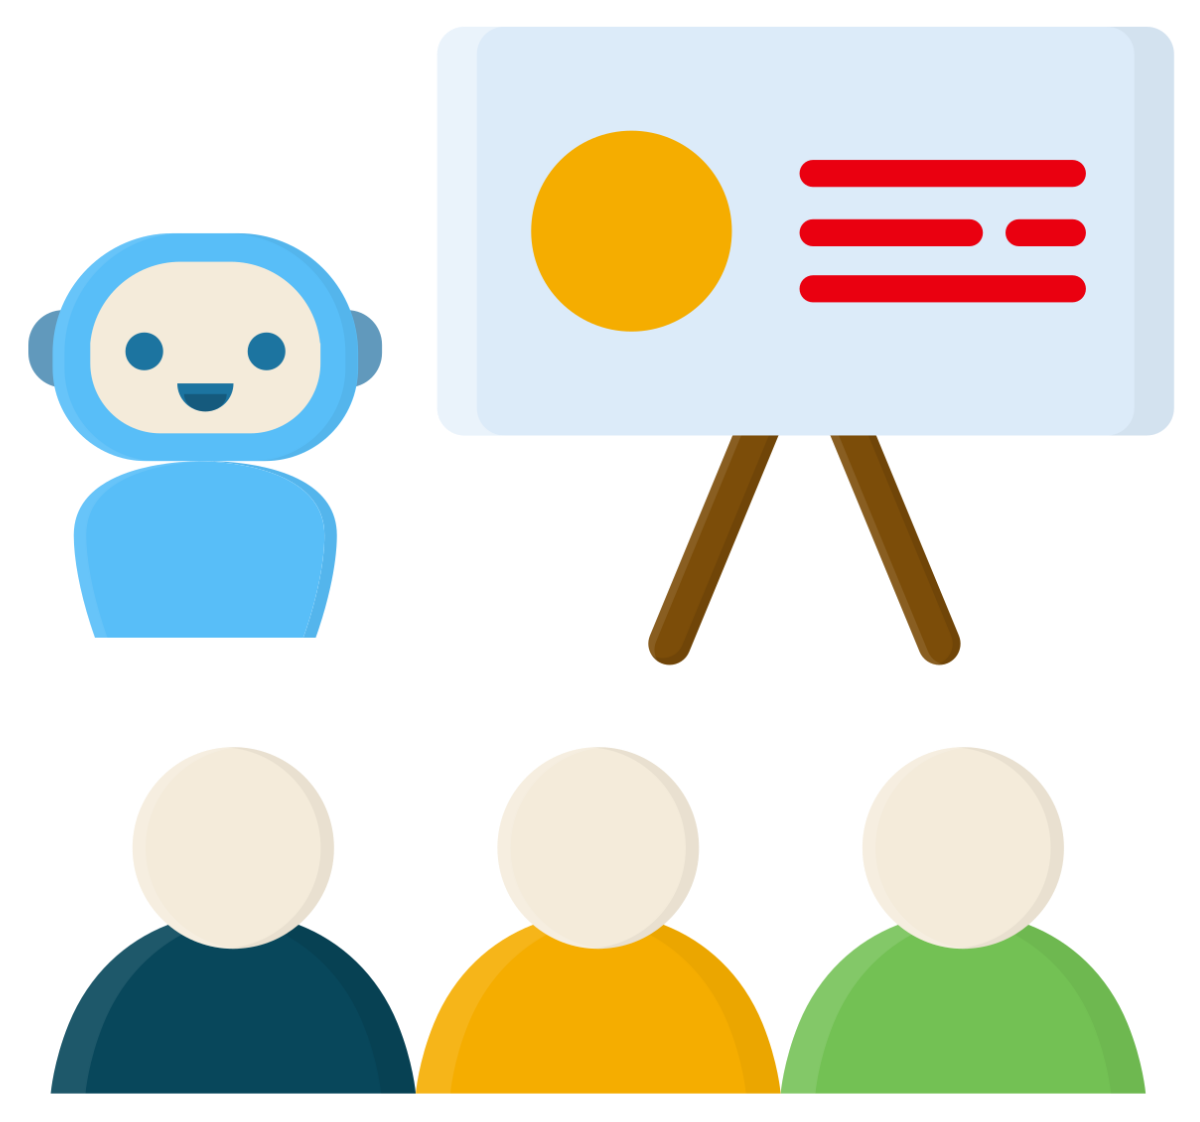
\includegraphics[width=0.15\textwidth]{Images/chapter_26/section_5683148496306176/5077119317966848.png}
 
\end{figure}

We have completed the class diagram of ESPNcricinfo according to the requirements. Now , let's design the sequence diagram of ESPNcricinfo in the next lesson.

% End of section content